\section{Diseño del modelo elástico}
\subsection*{Análisis del modelo elástico}

\addtocounter{framenumber}{-1}
\begin{frame}[t]{Contenidos}{\textcolor{UniBlue}{.}}
	\tableofcontents[currentsection]
\end{frame}

\begin{frame}[t]{Diseño del modelo elástico}{Análisis del modelo elástico}
\begin{itemize}
\item Recursos lógicos del sistema según el enfoque dinámico
\item Bajo overhead $\rightarrow$ Escalable
\item Técnica de fisión
\end{itemize}

\begin{picture}(0,80)
	\put(60,0){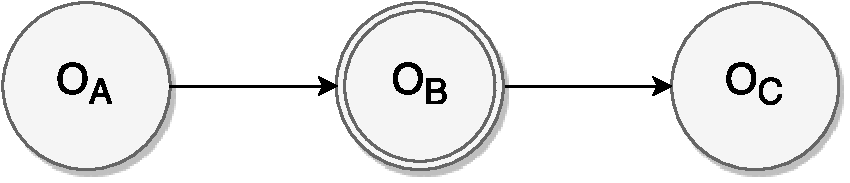
\includegraphics[scale=.5]{images/EjReplicacion-I.pdf}}
\end{picture}

\end{frame}

\addtocounter{framenumber}{-1}
\begin{frame}[t]{Diseño del modelo elástico}{Análisis del modelo elástico}
\begin{itemize}
\item Recursos lógicos del sistema según el enfoque dinámico
\item Bajo overhead $\rightarrow$ Escalable
\item Técnica de fisión
\end{itemize}

\begin{picture}(0,120)
	\put(60,0){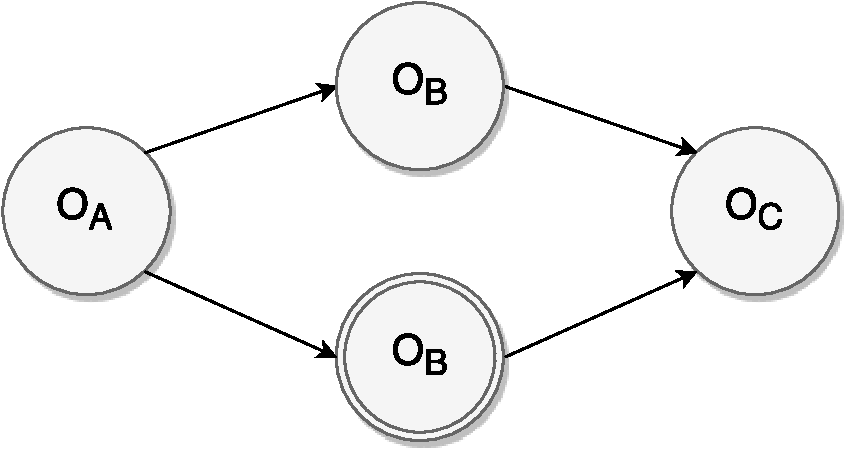
\includegraphics[scale=.5]{images/EjReplicacion-II.pdf}}
\end{picture}

\end{frame}

\addtocounter{framenumber}{-1}
\begin{frame}[t]{Diseño del modelo elástico}{Análisis del modelo elástico}
\begin{itemize}
\item Recursos lógicos del sistema según el enfoque dinámico
\item Bajo overhead $\rightarrow$ Escalable
\item Técnica de fisión
\end{itemize}

\begin{picture}(0,150)
	\put(60,0){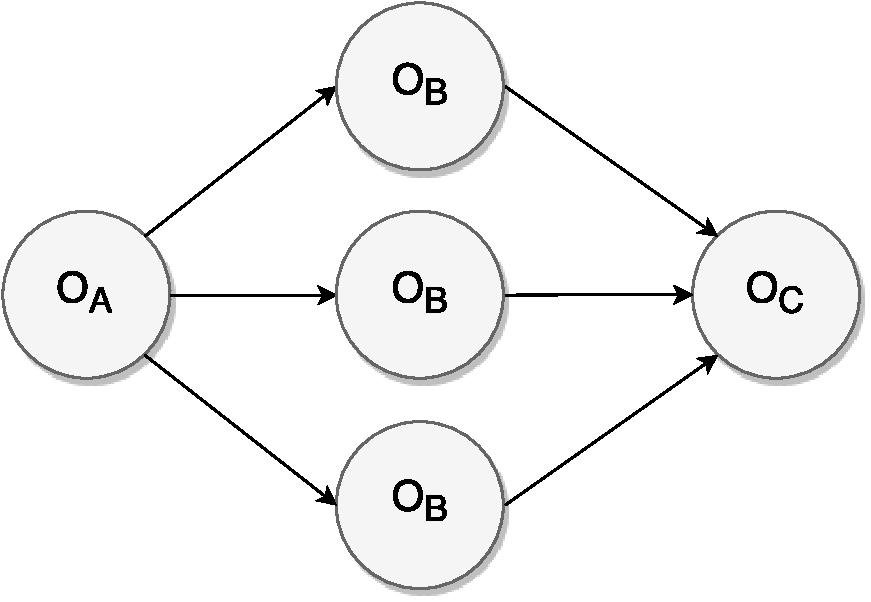
\includegraphics[scale=.5]{images/EjReplicacion-III.pdf}}
\end{picture}

\end{frame}

\begin{frame}{Diseño del modelo elástico}{Análisis del modelo elástico}
\begin{itemize}
\item Umbrales $\rightarrow$ Tasa de rendimiento $\rho$
	\begin{itemize}
		\item $\rho = \frac{\lambda}{s \mu}$
	\end{itemize}
\end{itemize}

\begin{figure}[!hb]
	\centering
	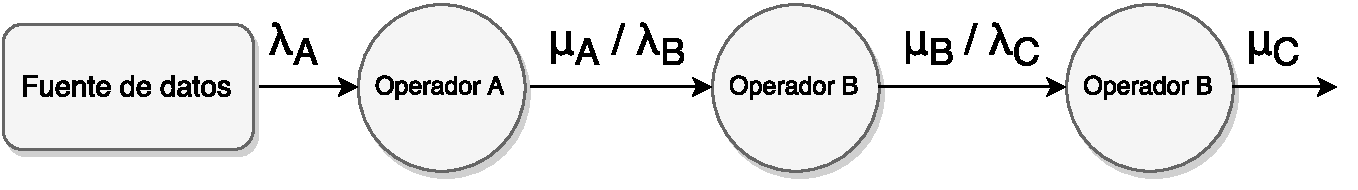
\includegraphics[scale=0.35]{images/AnalisisTeoriaColas.pdf}
\end{figure}

\begin{itemize}
\item Enfoque dinámico y elasticidad
\begin{itemize}
	\item Estados: ocioso, estable e inestable
\end{itemize}
\item Dos tipos de algoritmos: reactivo y predictivo
\item Recolector de datos y administrador de réplicas
\end{itemize}
\end{frame}

\begin{frame}{Diseño del modelo elástico}{Análisis del modelo elástico}
\begin{figure}[ht!]
  \centering
    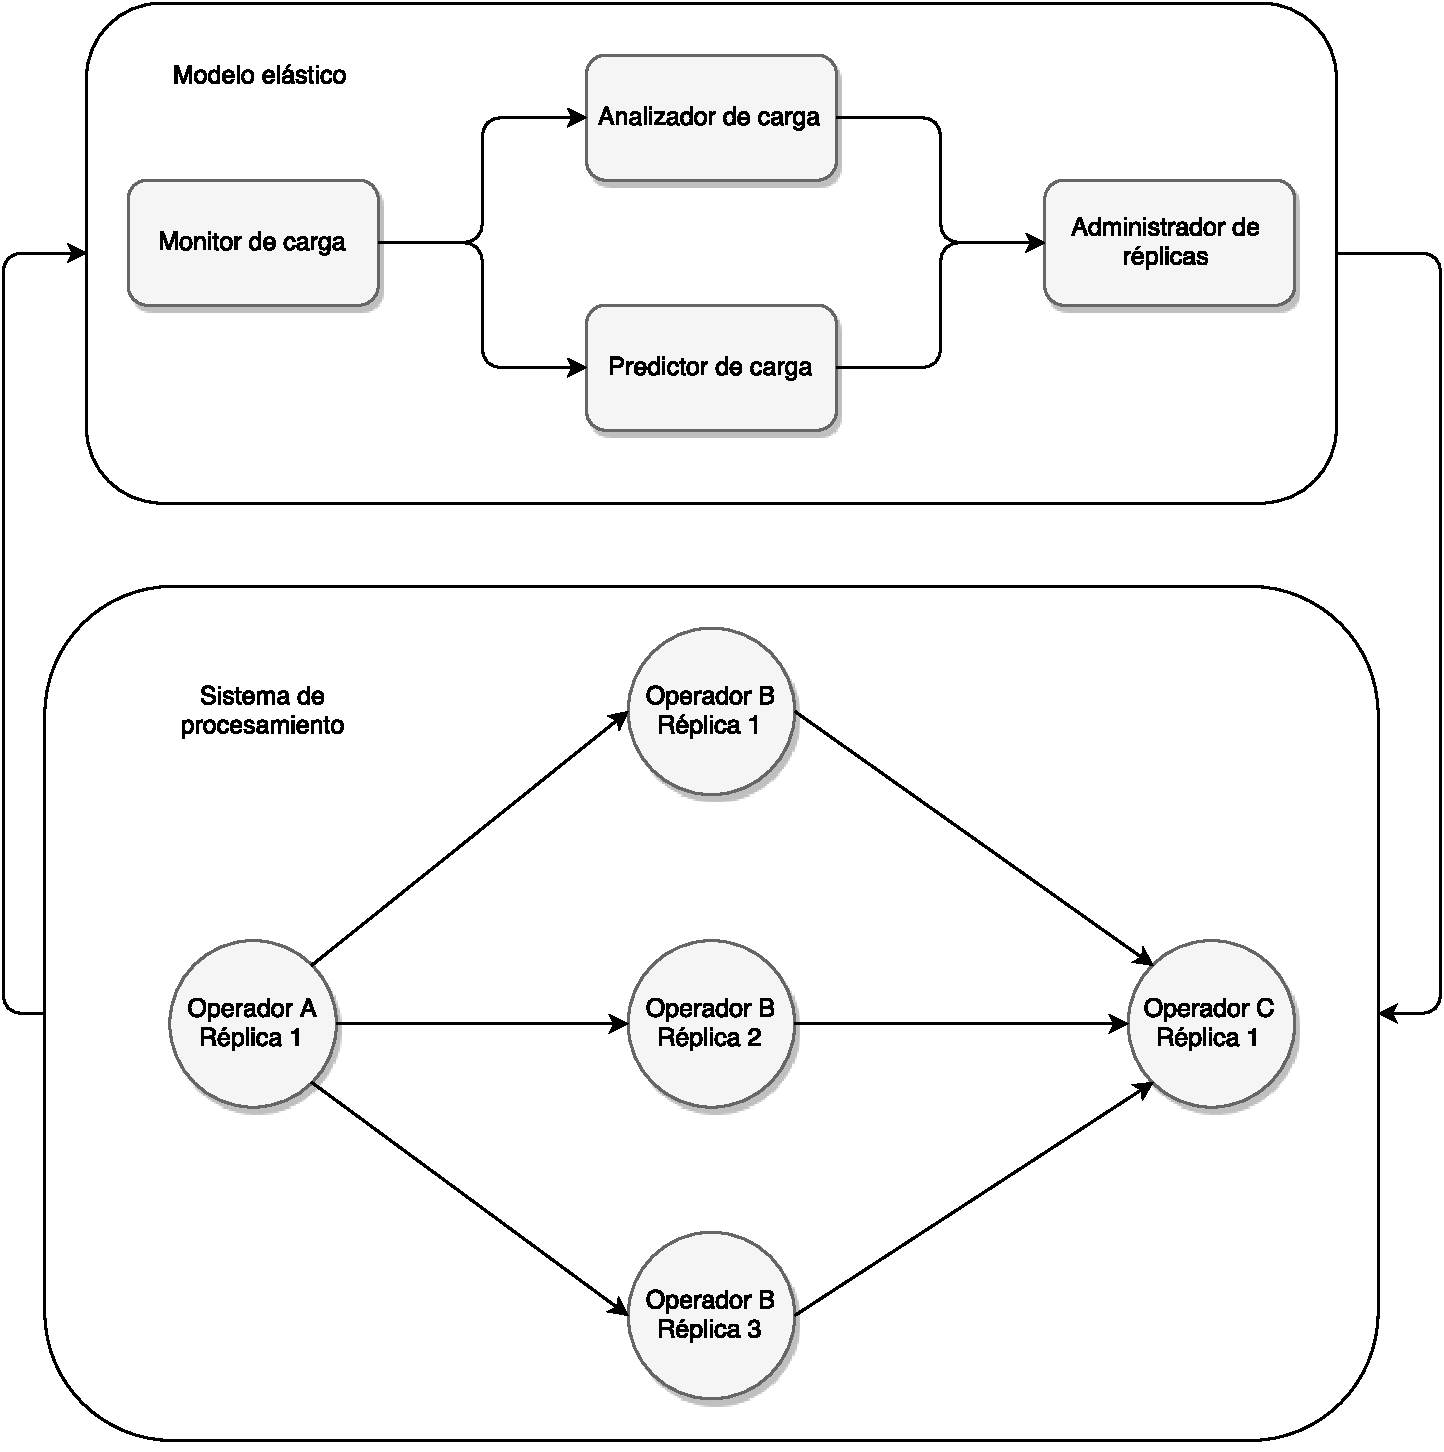
\includegraphics[scale=0.3]{images/Diagrama.pdf}
\end{figure}
\end{frame}

\subsection*{Recolección de los datos}
\begin{frame}{Diseño del modelo elástico}{Recolección de los datos}
El monitor de carga es el encargado de recolectar los datos
\begin{itemize}
	\item Algoritmo reactivo $\rightarrow$ Tasa de procesamiento $\rho$
	\begin{itemize}
		\item Tasa de rendimiento $\mu$ es homogénea
		\item Ventana de tiempo $T_r$
	\end{itemize}
	\item Algoritmo predictivo $\rightarrow$ Historial
	\begin{itemize}
		\item Ventanas de tiempo de $T$
		\item $n$ muestras
		\item Ventana de tiempo $T_p$
	\end{itemize}
\end{itemize}

\end{frame}

\subsection*{Algoritmo reactivo}
\begin{frame}{Diseño del modelo elástico}{Algoritmo reactivo}
\begin{itemize}
\item Análisis del estado del operador $\rightarrow$ Período de tiempo
\item Tasa de rendimiento $\rho$
\end{itemize}
\hspace{1cm}
\begin{tabular}{c c}
	$\rho > 1$ & Inestable \\
	$1 \geqslant \rho \geqslant 0.5$ & Estable \\
	$\rho < 0.5$ & Ocioso
\end{tabular}
\end{frame}

\begin{frame}{Diseño del modelo elástico}{Algoritmo reactivo}
\begin{itemize}
\item Comportamiento de la tasa de rendimiento
\end{itemize}
\begin{figure}[ht!]
  \centering
    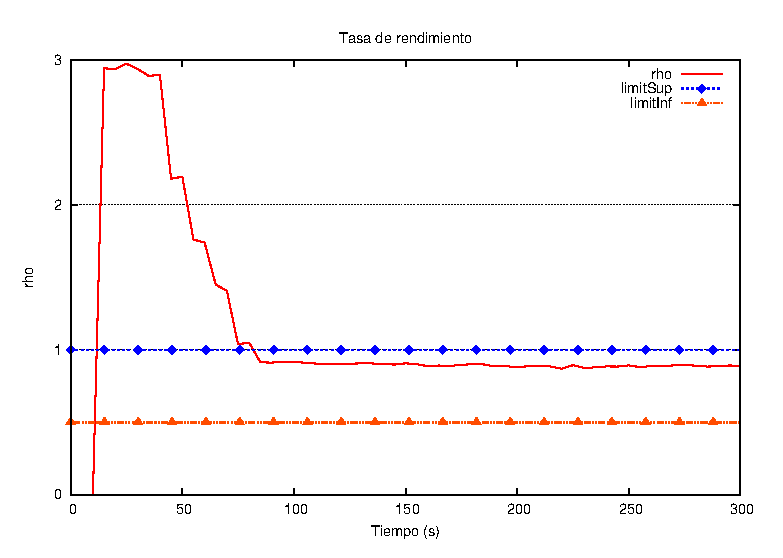
\includegraphics[scale=0.6]{images/Umbrales.eps}
\end{figure}
\end{frame}

\subsection*{Algoritmo predictivo}
\begin{frame}{Diseño del modelo elástico}{Algoritmo predictivo}
\begin{itemize}
	\item Definir muestras en tiempos discretos, las cuales cambian con el tiempo según un proceso estocástico
	\item Determinar los estados finitos que se utilizan para la conformación de la cadena
	\item Obtener una cantidad representativa de muestras para la construcción de la cadena de Markov en el período analizado
\end{itemize}

\begin{figure}[ht!]
  \centering
    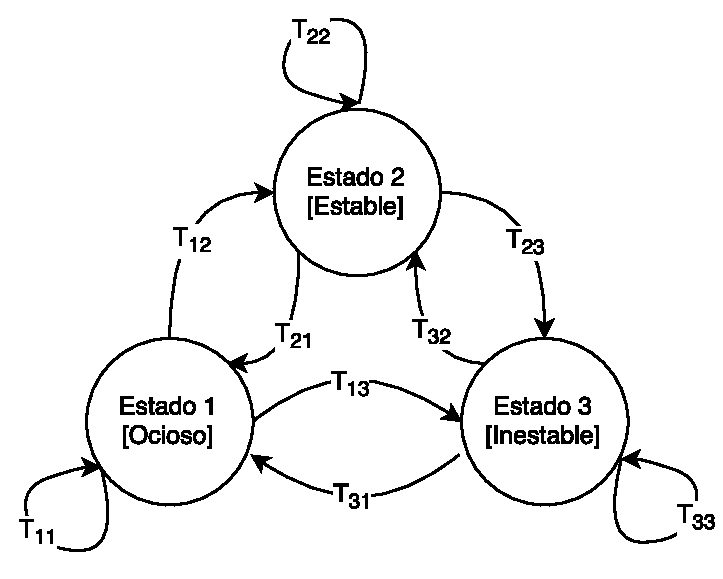
\includegraphics[scale=0.35]{images/CadenaMarkovPredictiva.pdf}
\end{figure}

\end{frame}


\begin{frame}{Diseño del modelo elástico}{Algoritmo predictivo}
\begin{itemize}
	\item Construcción de la matriz de transición
		\begin{itemize}
			\item La transición de estados de un período a otro
		\end{itemize}
\end{itemize}
\vspace{-1cm}
\begin{center}
\begin{align*}
	P =
	\begin{bmatrix}
		T_{1,1} & T_{1,2} & T_{1,3} \\
		T_{2,1} & T_{2,2} & T_{2,3} \\
		T_{3,1} & T_{3,2} & T_{3,3}
	\end{bmatrix}	
\end{align*}
\end{center}

\begin{itemize}		
	\item Ecuación de Chapman-Kolmogórov $\rightarrow$ Distribución Estacionaria
	\begin{itemize}
		\item Comportamiento a futuro de la Cadena de Markov
	\end{itemize}
\end{itemize}
\vspace{-1cm}
\begin{center}
\begin{align*}
\begin{bmatrix}
	\Pi_1 & \Pi_2 & \Pi_3
\end{bmatrix} _{(t+1)}
\end{align*}
\end{center}
\vspace{-0.5cm}
\begin{itemize}		
	\item $\sigma(\Pi_1, \Pi_2, \Pi_3) > 0.25$
	\begin{itemize}
		\item No posee incertidumbre
		\item En caso contrario, no es un comportamiento determinante
	\end{itemize}
\end{itemize}
\end{frame}

\subsection*{Administración del sistema}
\begin{frame}{Diseño del modelo elástico}{Administración del sistema}
\begin{itemize}
\item Administración de réplicas de un operador
\item Recursos disponibles de la máquina
\item Según el período se ejecuta
\begin{itemize}
	\item $T_p \rightarrow $ Algoritmo predictivo
	\begin{itemize}
		\item Menor frecuencia
		\item Mayor cómputo
		\item Modifica mayor cantidad de réplicas
	\end{itemize}
	\item $T_r \rightarrow $ Algoritmo reactivo
	\begin{itemize}
		\item Dos alertas $\rightarrow$ Modifica
	\end{itemize}
\end{itemize}
\end{itemize}
\end{frame}